\section{Motivation}
\label{sec:motivation}

Crowdsourcing platforms has been extremely well studied by different communities~\cite{doan2011crowdsourcing}.
We believe that they are harbingers of the oncoming shift towards the gig economy
brought upon by online job platforms.
By studying how workers fare in these platforms allows us to extrapolate the findings to Future of Work (FoW).

Crowdsourcing platforms including Amazon Mechanical Turk (AMT) and CrowdWorks have a number of similarities
to online job platforms.
Requestors create various tasks that include information such as description of the work required, compensation provided, requestor details etc.
The requestor can also filter workers based on previous experience.
When a worker logs on, she could see all the available tasks and choose to work on a subset of them.
When the worker submits a task, it could be reviewed by the requestor.
If deemed satisfactory, the worker is paid.
If not, the worker submission is rejected.
The crowdsourcing platform takes a cut from the payment made by requestor to the worker.
This basic model pioneered by AMT has become ubiquitous
in online job platforms as diverse as Uber, TaskRabbit and so on.

A number of studies such as~\cite{brawley2016work} have found that there is a large turnover
among workers in Crowdsourcing platforms.
Often, the barriers for turnover is much less steeper than in a traditional employment setting.
This often causes workers to either completely stop working in a platform such as AMT
or have a partial turnover where they just stop working on tasks from a particular requestor.
It is important to address both types of turnover.
The former could be illustrative of dissatisfaction with the platform
whereas the latter could be due to dissatisfaction with requestors.

We collaborated with CrowdWorks, one of the largest crowdsourcing platforms in Japan.
It provides support for more than 200 types of tasks.
%\red{More details about Crowdworks that could be relevant.}
It is used by more than 25000 companies and close to a million active workers. 
We begin by analyzing the turnover rate of workers in CrowdWorks. 
Figure~\ref{fig:persistenceRate} shows what fraction of workers
persist with the platform over a period of time.
One can see that as much as 75\% of workers drop off within couple of months.
The number of workers who persist for more than 2 years is as little as 5\%.
The success of any crowdsourcing platform hinges on successfully retaining workers.
Hence, identifying the factors causing worker turnover and mitigating them is of paramount interest.
It is expected that workers who drop-off have a wide variety of reasons for doing so.
We are specifically interested in the role of platform design for this phenomenon.
By understanding how workers feel about current platforms and their desiderata for new functionalities,
one can perform a better platform design. 

 \begin{figure}
    \centering
     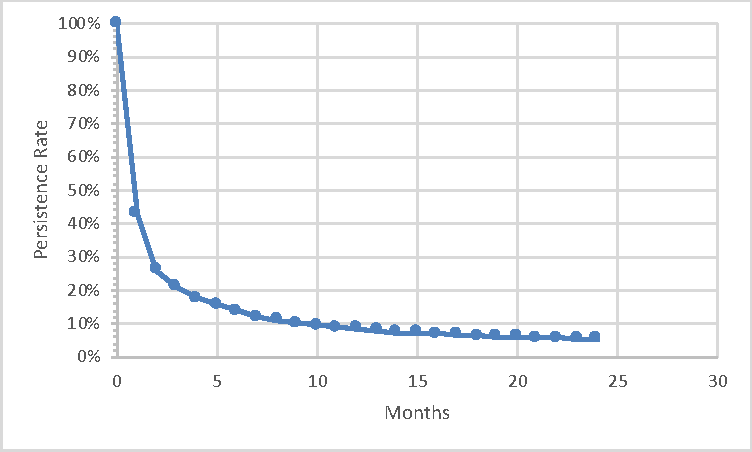
\includegraphics{figures/persistenceRateCrowdworks.pdf}
     \caption{Persistence Rate of Workers in CrowdWorks, according to the log of all workers who made accounts from January 1st, 2017 to December 31th, 2018.
     %\red{I hope this is okay to put in the paper. The figure needs to be improved. David: For the legend, maybe Persistence Rate of Workers on Crowdworks (50 workers, year 2019)? }
     }
     \label{fig:persistenceRate}
 \end{figure}

In December 2019, we conducted a poll of crowd workers on AMT and CrowdWorks, that have different characteristics; AMT is a microtask-based crowdsourcing platform, and CrowdWorks provides a wide variety of task types, focusing on a a bit larger tasks such as writing articles and codes.
This involved 101 workers (51 AMT and 50 CrowdWorks workers).
 Figure \ref{fig:surveyresult1}  summarizes the answers to the following questions: (Q1) Do you envision switching between platforms in the next X months? (Q2) How easy/challenging is switching between the platforms? 
 The result clearly shows that there is a strong correlation between worker mobility and the easiness of switching between platforms.
 We assume that since AMT is a pure microtask platform and obtaining a good reputation is easier, more workers think switching is easy in AMT than in CrowdWorks.
 Figure \ref{fig:surveyresult2} shows that workers would like platforms to have many advanced features that are not necessarily fully supported by the current generation of platforms. It is interesting to see that many workers on CrowdWorks dislike the collaboration feature among workers. We have not pursued the reasons yet, but a possible cause is the difference in the granularity of tasks. 

\begin{figure}[t]
\centering
\begin{tabular}{|c|c|c|c|c|c|c|c|}
\hline
Q1&Platform&\multicolumn{5}{|c|}{Q2}&Total\\
\cline{3-7}
&&Very Easy & Easy& Neither & Difficult & Very Difficult&\\
\hline
Yes&AMT&14\%&47\%&12\%&0\%&0\%&73\%\\
&CrowdWorks&0\%&2\%&6\%&2\%&0\%&10\%\\
\hline
No&AMT&4\%&6\%&6\%&10\%&2\%&26\%\\
&CrowdWorks&6\%&18\%&48\%&16\%&2\%&90\%\\
\hline
\end{tabular}
\caption{Results of Questions 1 and 2. The result suggests a correlation between the worker mobility  and the easiness of switching among crowdsourcing platforms.}
\label{fig:surveyresult1}
\end{figure}

\begin{figure}
    \centering
\begin{tabular}{|l|c|c|c|c|}
\hline
Q3. Preference for the feature?&Platform&\multicolumn{3}{|c|}{Answers}\\
\cline{3-5}
&&Like&Dislike&I don't know\\
\hline
Displaying Credentials&AMT&90\%&4\%&6\%\\
\cline{2-5}
&CrowdWorks&62\%&20\%&18\%\\
\hline
Specifying/ Quantifying/ Learning Skills&AMT&86\%&6\%&8\%\\
\cline{2-5}
&CrowdWorks&68\%&18\%&14\%\\
\hline
Anonymity&AMT&75\%&18\%&10\%\\
\cline{2-5}
&CrowdWorks&66\%&18\%&16\%\\
\hline
Complex Workflows&AMT&67\%&20\%&14\%\\
\cline{2-5}
&CrowdWorks&42\%&12\%&46\%\\
\hline
Collaboration&AMT&84\%&4\%&12\%\\
\cline{2-5}
&CrowdWorks&28\%&42\%&30\%\\
\hline
\end{tabular}
    \caption{Whether workers would like platforms to support for the features or not}
    \label{fig:surveyresult2}
\end{figure}

%\red{TBD after we get the poll results.}
